% =====================================================================
%  SECTION 6 — Tightness against the Voigt--Reuss envelope
%  Draft 1. The competitive defence. Every number traceable to RESULTS.md.
% =====================================================================

\section{What the certificate adds: tightness beyond the analytic envelope}
\label{sec:tightness}

An amortized surrogate can be made to satisfy a guarantee cheaply. Keshav,
Herb and Fritzen's Voigt--Reuss network~\cite{Keshav2025}
predicts effective stiffness tensors for unseen microstructures and
guarantees, by spectral normalisation of a factorised parameterisation,
that every prediction lies inside the analytic Voigt--Reuss envelope in the
L\"owner sense, during training, at inference, and under gradient-based
design. That construction overlaps the present work on four axes
simultaneously: amortization, tensor-valued elasticity, L\"owner
bracketing, and differentiable certified design.

The distinction is what the guarantee is \emph{about}. The Voigt--Reuss
envelope is a function of the phase fractions alone. It therefore carries
no information about the arrangement of the phases, and a prediction
confined to it is guaranteed only to be physically admissible. A
variational certificate is computed from admissible trial fields for the
specific microstructure, and can be strictly tighter. If it is not, the
present construction reduces to the cheaper one, so this section reports
the measurement rather than the argument.

\subsection{Measured tightening}
\label{sec:tightness:measured}

Table~\ref{tab:tightening} reports the ratio of the Voigt--Reuss relative
width to the certified relative width, for microstructures the operator did
not see during training, with all certificates obtained by exact
integration.

\begin{table}[t]
\centering
\caption{Tightening relative to the Voigt--Reuss envelope on controlled
test microstructures, contrast $10$. Certificates by exact integration; the
final column reports L\"owner validity for the specified numerical model.}
\label{tab:tightening}
\resizebox{\textwidth}{!}{%
\begin{tabular}{llrrrc}
\toprule
physics & microstructure & Voigt--Reuss & certified & tightening & valid \\
\midrule
conductivity & disks (held out) & 83.0\% & 20.8\% & 4.0$\times$ & yes \\
conductivity & disks (held out) & 89.6\% & 25.8\% & 3.5$\times$ & yes \\
conductivity & disks (held out) & 94.0\% & 33.7\% & 2.8$\times$ & yes \\
conductivity & laminate (OOD)   & 86.3\% & 21.1\% & 4.1$\times$ & yes \\
conductivity & checkerboard (OOD) & 100.6\% & 43.2\% & 2.3$\times$ & yes \\
\midrule
\multicolumn{2}{l}{\emph{conductivity, median}} & & & \textbf{3.5$\times$} & \\
\multicolumn{2}{l}{\emph{elasticity, controlled synthetic median (12 held out)}} & & & \textbf{2.7$\times$} & \\
\multicolumn{2}{l}{\emph{elasticity, controlled synthetic median (3 seeds)}} & & & \textbf{2.2$\times$} & \\
\bottomrule
\end{tabular}}

\end{table}

Figure~\ref{fig:tightening} summarises these results. The scalar-conductivity
intervals are between two and four times narrower than the envelope,
including microstructures drawn from families absent from training. The
elasticity rows are controlled synthetic demonstrations of the same
certificate construction, not an externally labelled coverage or matched
competitor study.


\begin{figure}[t]
\centering
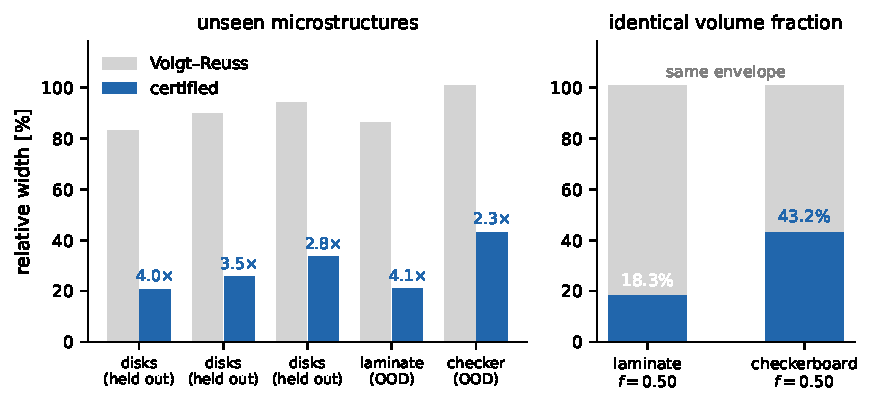
\includegraphics[width=\linewidth]{figures/fig_tightening.pdf}
\caption{Left: certified widths against the Voigt--Reuss envelope on unseen microstructures. Right: two microstructures of identical phase fraction receive the same envelope but certificates differing by more than a factor of two.}
\label{fig:tightening}
\end{figure}

\subsection{The envelope cannot distinguish geometry}
\label{sec:tightness:geometry}

The ratios above quantify the improvement; the following experiment
characterises its nature. Consider two microstructures with \emph{identical}
phase fractions and entirely different arrangements: a rank-one laminate at
volume fraction $0.500$, and a two-phase checkerboard at volume fraction
$0.500$.

\begin{table}[t]
\centering
\caption{Identical volume fraction, different geometry, conductivity at
contrast $10$. The Voigt--Reuss envelope is a function of phase fraction
alone and is therefore identical for both; the certified intervals differ
by more than a factor of two.}
\label{tab:geometry}
\resizebox{\textwidth}{!}{%
\begin{tabular}{lrrr}
\toprule
microstructure & volume fraction & Voigt--Reuss width & certified width \\
\midrule
laminate, $f = 0.50$ & 0.500 & 100.6\% & \textbf{18.3\%} \\
checkerboard         & 0.500 & 100.6\% & \textbf{43.2\%} \\
\bottomrule
\end{tabular}}
\end{table}

A guarantee derived from phase fractions assigns these two microstructures
the same admissible set, and must do so for any composite sharing their
composition. The variational certificate separates them by more than a
factor of two, and does so at inference cost. This is the difference
between a guarantee of physical admissibility and a certificate of
per-instance accuracy.

We note three honest qualifications. First, and most importantly, this
comparison is against the \emph{guarantee} that amortized surrogates
enforce, not against their point predictions, which may well be
considerably more accurate than the envelope they are constrained to. A
head-to-head against a trained surrogate's predictions is not attempted
here and would be a natural next study; the claim we make is about the
strength of the guarantee, and should not be read as a claim about
predictive accuracy. Second, the corresponding elasticity
experiment is far less striking: at the same volume fraction the certified
widths are $60.1\%$ (laminate) and $52.8\%$ (checkerboard) against a
$90.1\%$ envelope. Both test cases lie well outside the training family and
the elastic operator is the weaker of the two, so we present the
conductivity comparison as the primary evidence and report the controlled
synthetic elasticity figures alongside rather than in place of it. Third, a laminate is an
extremal microstructure: it attains the Voigt bound along the layers and
the Reuss bound across them, so its effective tensor lies \emph{on} the
envelope boundary in the principal directions and no method can be strictly
tighter there. The certified interval consequently need not be contained in
the envelope for laminates, which is a correct behaviour rather than a
defect.

\subsection{Summary of the comparison}
\label{sec:tightness:summary}

The three amortized approaches to guaranteed effective properties occupy
distinct positions:

\begin{center}
\resizebox{\textwidth}{!}{%
\begin{tabular}{lll}
\toprule
 & certificate & scope \\
\midrule
Gaynutdinova et al.~\cite{Gaynutdinova2026} & variational, tight & per-instance, scalar \\
Voigt--Reuss net~\cite{Keshav2025} & amortized, fraction-only & tensor elasticity \\
\textbf{this work} & \textbf{amortized and per-instance tight} & scalar and tensor, 2D \\
\bottomrule
\end{tabular}}
\end{center}

The contribution is the combination. Per-instance variational certificates
are tight but do not transfer; amortized envelope guarantees transfer but
carry no geometric information; the construction of
Section~\ref{sec:amortized} delivers certificates that transfer. On the
controlled scalar-conductivity study, they are two to four times tighter
than the envelope at inference cost. Section~\ref{sec:amortized:external}
adds an external elasticity coverage study, whose $1.05\times$ median
tightening is deliberately reported as modest; matched trained-predictor
comparisons remain future work.
